% This syllabus template was created by:
% Brian R. Hall
% Associate Professor, Champlain College
% www.brianrhall.net

% Document settings
\documentclass[11pt]{article}
\usepackage[margin=1in]{geometry}
\usepackage[pdftex]{graphicx}
\usepackage{multirow}
\usepackage{setspace}
\usepackage{enumitem}
\usepackage{longtable}
\setlist{nosep}
\pagestyle{plain}
\setlength\parindent{8pt}


\begin{document}

% Course information
\begin{tabular}{ l l }
  \multirow{3}{*}{
\includegraphics[width=2in]{Main-Logo-black.png}} & \LARGE CSCI447/547 \\
  & \LARGE Machine Learning \\
  & \LARGE TR, 12:30PM-2:00PM, SS 362\\
\end{tabular}
\vspace{7mm}

% Professor information
\begin{tabular}{ l l }
  \multirow{6}{*}{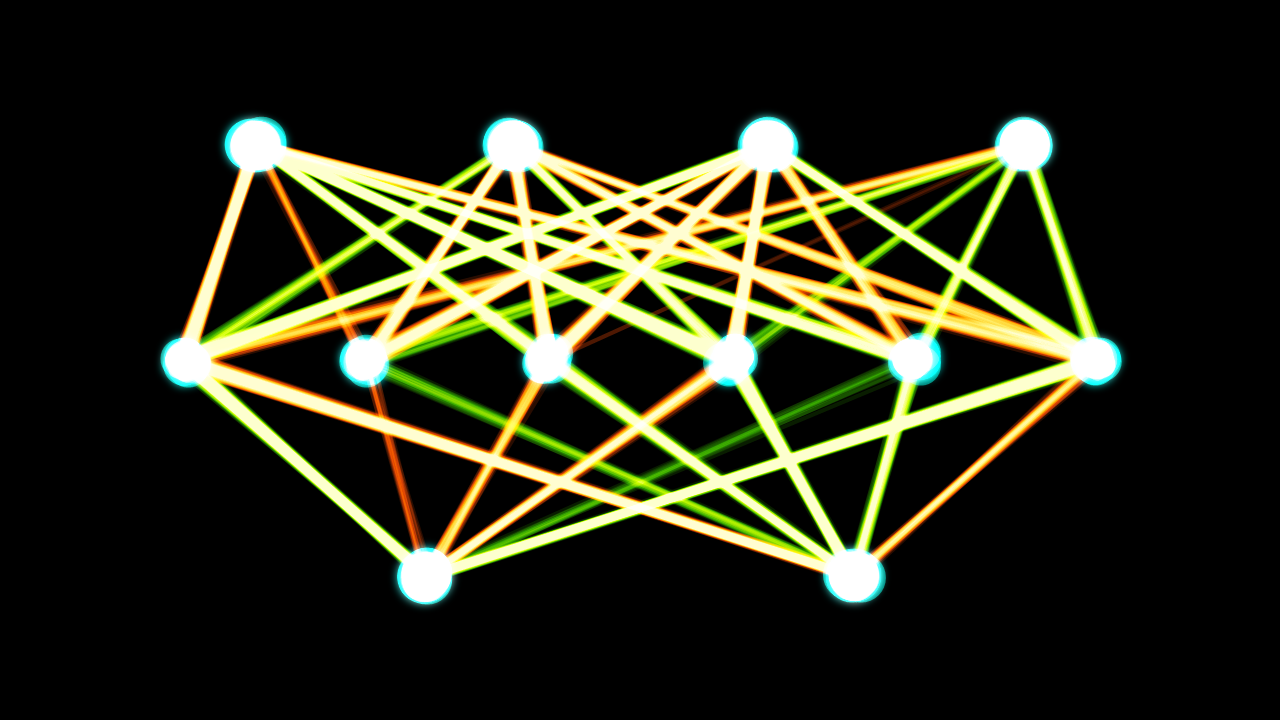
\includegraphics[height=1in]{nn.png}} & \large Instructor: Doug Brinkerhoff \\
  & \large E-mail: douglas1.brinkerhoff@umontana.edu \\
  & \large Office: SS403 \\
  & \large Office Hours: TWR, 11:00AM-12:30PM \\
	& (E-mail for an appointment, or my door is always open when I'm in.  You should feel welcome (encouraged!) to drop by.)\\
\end{tabular}
\vspace{5mm}

% Course details
\textbf {\large \\ Course Description:} As a society we have reached a point where the amount of information available to us exceeds our capacity to analyze it without the assistance of the very computers that have made the collection of such vast sums of data possible.  In this course we will explore the techniques required to turn these data into predictive models of varying complexity, from the modest linear regression to the vaunted deep neural network, with many other methods in between. \vspace{5mm} \\
\textbf{\large Course Objectives:} At the completion of this course, the successful student will be able to:
\begin{enumerate}
  \item Understand the language of machine learning in the context of contemporary data analysis.
  \item Understand fundamental principles such as inductive bias, overfitting, and uncertainty. 
  \item Select models appropriate for the structure and subject of problems being considered.
  \item Implement a bestiary of machine learning algorithms, both from scratch and with the assistance of high performance libraries like Google's TensorFlow.
\end{enumerate}
\textbf{\large Class Organization:} Class time will be mostly interactive lectures and the occasional collaborative in-class work session.  This course is taught in python, which is currently the most common language used in machine learning  
\vspace{5mm}\\
\textbf{\large Course Webpage:} In this course, all materials will be distributed via the version control software git.  The course webpage will then be a github `organization', which can be found at https://github.com/UMT-CS447-547-Fall-2018.  Course materials (e.g. this document, lecture notes, etc.) can be found as git repositories there.  Furthermore, assignments will be distributed via git and submitted as git pull requests (more on this in a separate document).  Grades will be recorded in Moodle.
\vspace{5mm}\\
\textbf{\large Student Evaluation:}
There will be fortnightly assignments on which you are encouraged to work with your classmates.  Grad students will have the enviable experience of answering an extra advanced problem on each assignment.  As stated above, these assignments will be distributed and submitted as ipython notebooks via the version control software git.  Note that by default, your work will be visible to your classmates, and theirs visible to you.  I encourage collaboration, and this is one way to facilitate that.  If you are uncomfortable with this, let me know and I will make your materials private, but you also lose access to your peers' submissions.  (Note that this collaborative environment may disappear if you are abusing the privilege!)

Each student will be required to propose and execute a project.  For undergraduates this may be either the implementation of a machine learning algorithm not covered in class, the application of machine learning to a non-trivial dataset, or an in depth report on a contemporary or classic academic paper on machine learning.  This last option will not be available to grad students.  This project will take the place of a final exam.  The grade breakdown is as follows: 70\% assignments, 20\% final project, 10\% project proposal.   
\vspace{5mm}\\
\textbf{\large Computers, Software, and Online Material:}
If possible, bring a laptop to class.  A tentative list of the software that we'll be using is as follows:
\begin{enumerate}
\item Python 3
\item Numpy/Scipy/Matplotlib: http://www.scipy.org/install.html
\item Jupyter: http://jupyter.org/install
\item scikit-learn: http://scikit-learn.org/stable/install.html
\item tensorflow: https://www.tensorflow.org/install/
\end{enumerate}

\textbf{\large Prerequisite(s):} Officially, CSCI232: Data Structures and Algorithms.  In reality, this course requires a commitment to making up any knowledge gaps that the student might have with respect to the course material.  Because of the nature of the subject, ML borrows heavily from topics in calculus, statistics, discrete math, and programming.  It is unlikely that anyone is going to be comfortable with the course material all the time.  Don't get too bent out of shape about it.  
\vspace{5mm} \\
\textbf {\large Text(s):} \begin{enumerate} \item \emph{Machine Learning: A Probabilistic Perspective}, Kevin P. Murphy, MIT Press, ISBN: 9780262018029 
\end{enumerate} \vspace{5mm}
\textbf {\large Letter Grade Distribution:} \\\\
\hspace*{40mm}
\begin{tabular}{ l l | l l }
\textgreater= 93.00 & A & 73.00 - 76.99 & C \\
90.00 - 92.99 & A-  & 70.00 - 72.99 & C- \\
87.00 - 89.99 & B+  & 67.00 - 69.99 & D+ \\
83.00 - 86.99 & B  & 63.00 - 66.99 & D \\
80.00 - 82.99 & B-  & 60.00 - 62.99 & D- \\
77.00 - 79.99 & C+  & \textless= 59.99 & F \\
\end{tabular} \\
\vspace{5mm} \\
\textbf{\large Late Assignments:}
I will not accept late assignments unless an extension was agreed upon well in advance of the due date or in extenuating circumstances to be determined at my discretion. \vspace{5mm} \\
\textbf{\large Academic Integrity:}
All students must practice academic honesty. Academic misconduct is subject to an academic penalty by the course instructor and/or a disciplinary sanction by the University. All students need to be familiar with the Student Conduct Code. I will follow the guidelines given there. In cases of academic dishonesy, I will seek out the maximum allowable penalty.  Polemic:  Look, this is a 400/500 level class, and if you're reading this you're probably looking to have a career in CS or a related field.  When you're at a job interview, don't be sitting there regretting that you didn't learn anything in Machine Learning because you were cheating the whole time.  Nobody wants that.  \vspace{5mm} \\
\textbf{\large Disabilities:}
Students with disabilities may request reasonable modifications by contacting me. The University of Montana assures equal access to instruction through collaboration between students with disabilities, instructors, and Disability Services for Students. Reasonable means the University permits no fundamental alterations of academic standards or retroactive modifications. \vspace{5mm} \\
% Course Outline
\textbf {\large Tentative Course Schedule:}
The following is subject to change according to the rate at which we proceed through the material, the moon and tides, and the results of my horoscope for the week.
\begin{longtable}{| l | p{6cm} | p{3cm} | p{3cm} | }
\hline
\textbf{Date} & \textbf{Topic} & \textbf{Assignments Assigned} & \textbf{Reading} \\
\hline
Aug. 27 -- Aug. 31 & What does it mean to learn? -- Basic probability & HW1& Ch.1 \\
Sep. 03 -- Sep. 07 & Graphical Models/Naive Bayes & Project Proposal & Ch. 2 \\
Sep. 10 -- Sep. 14 & Naive Bayes/Markov Models  & HW2& Ch. 10 \\
Sep. 17 -- Sep. 21 & Markov Models & & Ch. 17 \\
Sep. 24 -- Sep. 28 & Hidden Markov Models with Travis & HW3 & \\
Oct. 01 -- Oct. 05 & State Space Models with Jesse & & Ch. 18 \\
Oct. 08 -- Oct. 12 & Particle Filtering & HW4 & \\
Oct. 15 -- Oct. 19 & Mixture Models/Expectation Maximization & Project & Ch. 11\\
Oct. 22 -- Oct. 26 & Model Selection/PCA & HW5 & Ch. 12 \\
Oct. 29 -- Nov. 02 & Linear Regression/Logistic Regression & & Ch.7 \\
Nov. 05 -- Nov. 09 & Feedforward Neural Networks & HW6 & Ch. 16.5 \\
Nov. 12 -- Nov. 16 & Backpropagation/Regularization & & Course notes \\
Nov. 19 -- Nov. 23 & Tensorflow & HW7 & Google's docs \\
Nov. 26 -- Nov. 30 & Convolutional Neural Networks & & \\
Dec. 03 -- Dec. 07 & Recurrent Neural Networks & & \\
\hline
\end{longtable} 

\end{document}



